% Chapter Template

\chapter{Recommendation Engine}% Main chapter title
\label{Chapter6} % Change X to a consecutive number; for referencing this chapter elsewhere, use \ref{ChapterX}


The quality of the recommendation system design determines the quality of the posts recommended to our users. 
A recent study by Epsilon found that 90\% of consumers find personalisation appealing. Plus, a further 80\% claim they are more likely to cooperate with a company when offered personalised experiences.
The study also found that these consumers are ten times more likely to become VIP customers, who make more than 15 purchases per year.\footfullcite{epsilon} 
Thus a well-designed recommendation system can benefit the monetisation of our app in the future.
\\Recommendation systems are divided into personalised and non-personalised ones, where personalised recommendation systems can be further divided into content-based filtering systems and collaborative filtering systems. 
The overview of recommendation system can be seen in figure \ref{fig:overrecomm}.
\begin{figure}[ht]
\centering
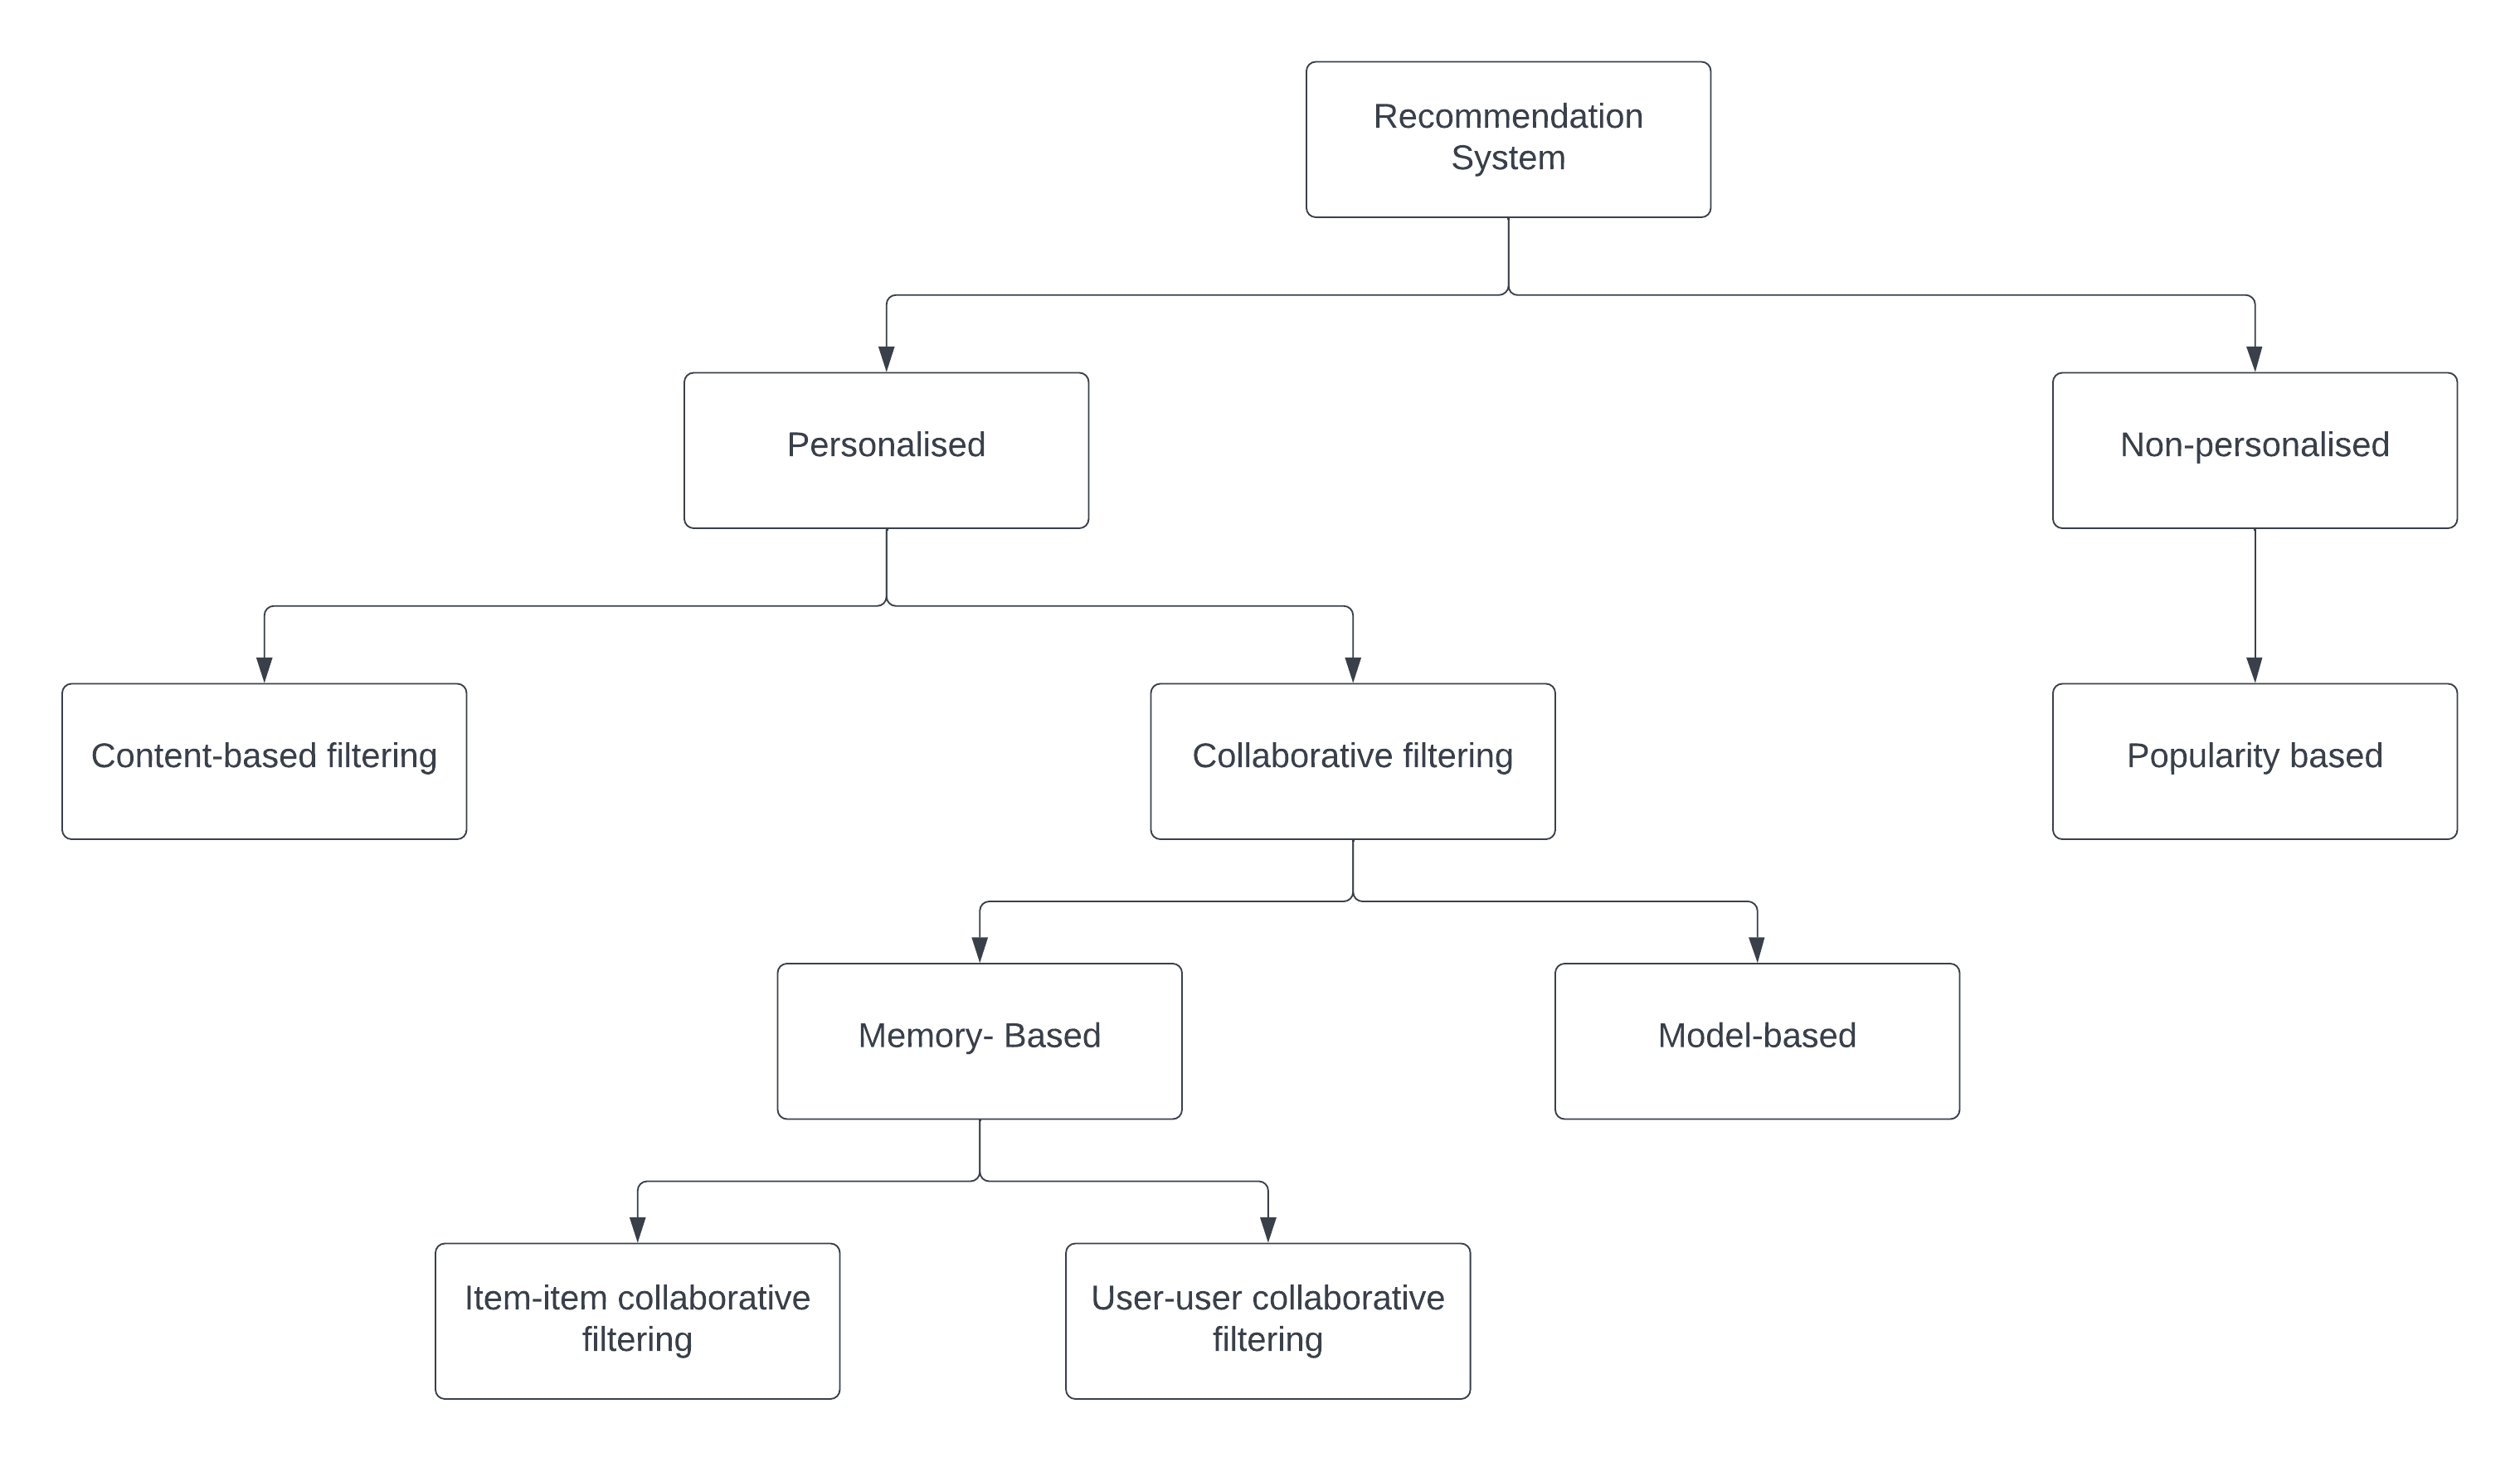
\includegraphics[scale = 0.13]{overview11.png}
\caption{Overview of recommendation system}
\label{fig:overrecomm}
\end{figure}

%-----------------------------------------------------------------------------------------------------------------------------Popularity-Based Recommendation System
\section{Popularity Based Recommendation System}
It is a type of recommendation system which works on the principle of popularity and or anything which is in trend. These systems check the product or movies which are in trend or are most popular among the users and directly recommend those. 
Instead of recommending posts only based on the number of likes that the posts received, we can give weighting to each parameter involved in our decision and one of the weighted rating system examples is shown below.
\begin{equation}
\textbf{Rating}(v,m,R,C) = \frac{v}{v+m} \times R + \frac{m}{v+m} \times C
\end{equation}
Where:
\\$R$ is the average rating for the item.
\\$v$ is the number of votes for the item.
\\$m$ is the minimum votes required to be listed in the popular items(defined by > percentile 80 of total votes).
\\$C$ is the average rating across the whole dataset.
\\This example is used to calculate rating scores by IMDB, which is an online database of information related to films and television series.
Inspired by the example above, we can introduce non-linearity in algorithms to calculate the scores of the posts to build our popularity-based recommendation system.
We want to construct $f(L,C,m,g)$, where $L$ is the number of likes the post received, $C$ is the number of comments the post received, 
$m$ is the minimum of likes to be listed as a popular item, $g$ is the gradient of change in the number of likes in w.r.t time in recent period time.
\\The most obvious disadvantage of a popularity-based system is the non-personalisation.




%-----------------------------------------------------------------------------------------------------------------------------Content-Based Recommendation System
\section{Content Based Recommendation System}
\label{Content Based Recommendation System}
Content-Based Recommendation Systems are based on a description of the item and a profile of the user's preferences. 
These methods are best suited to situations where there is known data on an item (name, location, description, etc.), but not on the user. 
Content-based recommenders treat recommendation as a user-specific classification problem and learn a classifier for the user's likes and dislikes based on an item's features.
\\ Before we can dive into the algorithm, we must assume that there are available features that captures the content of the item.
\\ First we need to obtain the post-feature matrix (table:\ref{itemfea}).
\begin{table}[ht]
\centering
\begin{tabular}{ |c|c|c|c|c|c|} 
 \hline
 \diagbox{Posts}{Features}&Feature1&Feature 2&Feature 3&$\cdots$&Feature $j$\\
 \hline
 Post1&&&&&\\
 \hline
 Post2&&&&&\\
 \hline
 $\vdots$&&&&&\\
 \hline
 Post $i$&&&&&\\
 \hline
 \end{tabular}
 \caption{Post Feature Matrix}
 \label{itemfea}
 \end{table}
\\The ratings given in the table measures the degree of the features in the posts, and we can assume the matrix is not sparse, which we mean the matrix is fully filled.
\\We denote that each row is the feature vector $x(i)$ for post $i$.
%
\\In addition, we need to get the profile of each users, which means we need to know and analyze the preference of our users, 
so we need to obtain the user parameter vector for each user and it reflects how the user responds to the features.
%
\\After we have the post-feature matrix and user parameter vector $\theta(j)$ of user j, we apply similarity metrics, here we use cosine similarity to measure 
the resemblance between $\theta(j)$ and each $x(i)$ in the post-feature matrix.
\\Cosine Similarity:  As the name mentioned, It measures the cosine angle of the two vectors in the multi-dimensional space. Two things can be similar together in terms of direction rather than magnitude.
\begin{equation*}
\text{Cosine Similarity} = cos(\theta) = \frac{A \cdot B}{||A|| ||B||}
\end{equation*}
\\Our system can then recommend posts to our user$j$ based on the similarity scores.
\\The biggest problem here in our design is how can we determine the subjective features of the content, such as genre, vibe, mood, and etc. Our current solution to this problem is including "tags" in the posts, and give limit number of choices for our users to choose from, 
and a percentage meter to indicate the degree of the features for them to set. Therefore the post-feature metrix will intensively rely on our users and it can suffer from subjectiveness.
However, we believe this design gives our users more freedom and space to show the feelings behind their songs.
\\Content based models are most advantageous for recommending items when there is an insufficient amount of rating data available. This is because other items with similar attributes might have been rated by the user. Hence, a model should be able to leverage the ratings along with the item attributes to generate recommendations even when there isn’t a lot of data.
There are some disadvantages of content-based approach as well, they are ineffective for providing recommendations for new users. 
The solution to it can be throigh an UX/UI deisgn, which is inspird by Apple Music, YouTube Music and Xiaohongshu, we would pop out a page for our users to choose preference from given choices, the bubbles will have 3 sizes to indicate 'interested in', 'like' and 'very like' levels of preferences. 
This solves the problem with the initialisation of user parameter vector. 
Another disadvantage can be that when building a model you require a history of explicit / implicit user level data for the items. It’s generally important to have a large dataset of ratings available to make robust predictions without overfitting.
\\The recommendations provided are “obvious” based on the posts / content the user has consumed. This is a disadvantage because if the user has never interacted with a particular type of post, that type will never be recommended to the user. 
For example, if the user has not seen any sad song post , then through this approach, he will never be recommended sad song posts. This is because the model is user specific and doesn’t leverage knowledge from similar users. This reduces the diversity of the recommendations, this is a negative outcome for many businesses.
\\Also people's perference will change, considering user experience, we can not ask our users to update their preference everyday or everyweek, 
and most of the time, users don't know their prefernece clearly as well. Thus being difficult to update user parameter vector is also one of the drawbacks in this approach.

%-----------------------------------------------------------------------------------------------------------------------------Collaborative Recommendation System
\section{Collaborative Filtering Recommendation System}
Collaborative filtering is the process of predicting the interests of a user by identifying preferences and information from many users. 
This is done by filtering data for information or patterns using techniques involving collaboration among multiple agents, data sources, etc. 
The underlying intuition behind collaborative filtering is that if user A and B have similar taste in a product, then A and B are likely to have similar taste in other products as well.
It has a interesting property, feature learning which is that it can learn for itself what features to use. 
\\We can divide collaborative filtering system into model-based approach and memory-based approach, and the memory-based approach can 
further be divided into item-based and user-based systems.
\\Before we dive into algorithm, we first need to construct the user-item interaction matrix \autoref{fig:UtilityM}.
\begin{table}[ht]
\centering
\begin{tabular}{ |c|c|c|c|c|c|} 
 \hline
 \diagbox{Items}{Users}&User 1&User 2&User 3&$\cdots$&User $j$\\
 \hline
 Item1&&&&&\\
 \hline
 Item2&&&&&\\
 \hline
 Item3&&&&&\\
 \hline
 $\vdots$&&&&&\\
 \hline
 Item $i$&&&&&$y^{(i,j)} \text{ if } r(i,j) = 1$\\
 \hline
 \end{tabular}
 \caption{User-Item Interaction Matrix}
 \label{fig:UtilityM}
 \end{table}
\\We denote that:
\\$r(i,j) = 1$,  if user $i$ rated item $j$ ( $0$,  otherwise.)
\\$y^{(i,j)}$ \text{is the rating by user $j$ on item $i$}
\\The first question will be faced in this approach is how we can get ratings $y^{(i,j)}$. The music posts are different from the movie rating system, considering our user experience,
we cannot ask our user to rate each post, the more sensible way is to allow them give "Like"s. However, inspired by a Chinese video-streaming app, Bilibili, we can make some changes to the "like" system. 
Instead of "like" or "not give like", we introduce a "super like" that our user can give to a post by 'press and hold' on the 'like' button .
\\Now we want to construct a rating function $y^{(i,j)}(L,t,S,T)$
\\Where
\\$L$ is 0 if "no like is given", 1 if "liked" and 2 if "super liked".
\\$t$ is the time our user spent on the post. Since we are not introducing a "dislike" feature in posts which will discourage our users to share their works,
 so we will set a threshold value for indicting "dislike". For example, if a user spends 3 seconds, below the threshold value, on a post and then exits, then the system will turn $L$ into "-1".
\\$S$ is 0 if the post has not been saved by the user and 1 if the post is saved by user.
\\$T$ is how many times the user$j$ have watched post$i$, currently.
\\Formulating the equation can be another problem, like in machine learning, we need data to fit our model or function into, which means we need to get some ratings to test or validate our rating function. 
Hence we will randomly selects small portion of posts to ask our user to rate.


%-----------------------------------------------------------------------------------------------------------------------------Memory-based CF
\subsection{Memory Based Approaches}
Memory based approaches are also often referred to as neighbourhood collaborative filtering. Essentially, ratings of user-item combinations are predicted on the basis of their neighbourhoods. 
This can be further split into user based collaborative filtering and item based collaborative filtering. 
User based essentially means that likeminded users are going to yield strong and similar recommendations. Item based collaborative filtering recommends items based on the similarity between items calculated using user ratings of those items.
\\The memory-based approach is so simple that it calculates the similarity matrix directly from the user-item matrix. There are two branches in memory based approaches, Item-based collaborative filtering and user-based collaborative filtering.

\subsubsection{Item-based Collaborative Filtering}
\\This method was first invented and used by amazon in 1998. 
Rather than matching the user to similar customers, item-to-item collaborative filtering matches each of the user’s purchased and rated items to similar items, then combines those similar items into a recommendation list. Now, let us discuss how it works.
\\Instead of applying cosine similarity, the better approah will be using pearson correlation coeffient
\\\textbf{Pearson Correlation}: The most well-known similarity metric for the linear relation is person correlation. It measures how similar two samples are based on the direction of how the value changes. 
The method for finding the similarity between two vectors is also called \textbf{Centred Cosine Similarity}. The word "Centred" means we will normalise utility matrix first by subtracting row mean, it solves the problem when we made the assumption by assuming unrated item by user will be rated 0. 
\begin{equation*}
\text{Pearson Correlation Coefficient} = \frac{\sum(x_{i} - \bar{x})(y_{i} - \bar{y})} {\sqrt{\sum(x_{i} - \bar{x})^{2} \sum{(y_{i} - \bar{y})^{2} }}}
\end{equation*}
\\We find the group of similar items based on users' similarity metric choice.
\\Select up to the top-k most similar item to recommend. \autoref{}


\subsubsection{User-based Collaborative Filtering}
\\We find the group of similar users (the group size is arbitrary) based on pearson correlation similarity metric.
\\We average the rating of each item based on the group of similar users
\\Rank the item based on the descending average rating, and recommend the target user with the item they never interacted with before.


%-----------------------------------------------------------------------------------------------------------------------------Model-based CF
\subsection{Model Based Approaches}
Model based approaches are predictive models using machine learning. Features associated to the dataset are parameterised as inputs of the model to try to solve an optimisation related problem. 
Model based approaches include using things like decision trees, rule-based approaches, latent factor models etc.
\subsubsection{Optimisation Algorithm}
\\First we need to construct the user-post iteraction matrix \autoref{fig:UtilityM}
\begin{enumerate}

\begin{table}[ht]
\centering
\begin{tabular}{ |c|c|c|c|c|c|} 
 \hline
 \diagbox{Posts}{Users}&User 1&User 2&User 3&$\cdots$&User $j$\\
 \hline
 Post1&&&&&\\
 \hline
 Post2&&&&&\\
 \hline
 Post3&&&&&\\
 \hline
 $\vdots$&&&&&\\
 \hline
 Item $i$&&&&&$y^{(i,j)} \text{ if } r(i,j) = 1$\\
 \hline
 \end{tabular}
 \caption{User-Post Interaction Matrix}
 \centering
 \end{table}

\item  Obtain a set of features folder, each measuring the degree of the content.
Denote that:
\\$r(i,j) = 1$,  if user $j$ rated item $i$ ( $0$,  otherwise.)
\\$y^{(i,j)}$ \text{is the rating by user $j$ on item $i$}
\\$\theta^{(i)}$ \text{is the parameter vector of user $j$}, which is called a latent-fatcor
\\$x^{(j)}$ \text{is the feature vector of item $i$}, which is call a latent-factor
\\$m^{(j)}$ \text{is the number of items rated by user $j$}
\\We want to reconstructed the matrix and compute the absent ratings using matrix factorisation \autoref{Matrix Factorisation}, then the predicted rate on the item $i$ by user $j$ is $(\theta^{(i)})^{T}(x^{(j)})$
\item Treat predicting the ratings of each user as a separate linear regression problem.
\item Minimise the square error term.
\end{enumerate}

Thus if we want to learn $\theta^{(i)}$ for user $j$:

\begin{equation*}
\min_{\theta^{(j)}} \frac{1}{2m^{(j)}}\sum_{i:r(i,j) = 1}\left((\theta^{(i)})^{T}x^{(j)}-y^{(i,j)}\right)^{2} + \frac{\lambda}{2m^{(j)}}\sum_{k = 1}^{n}(\theta^{(i)}_{k})^{2}
\end{equation*}
\\Where the last term is the usual regularisation term to prevent the overall equation to go to infinity and to prevent overfitting.
\\ To learn $\theta^{(1)}$,$\theta^{(2)}$, \dots, $\theta^{(j)}$:
\begin{equation*}
\min_{\theta^{(1)},\theta^{(2)}, \dots, \theta^{(j)}} \frac{1}{2}\sum_{j = 1}^{n_{u}}\sum_{i:r(i,j) = 1}\left((\theta^{(i)})^{T}x^{(j)}-y^{(i,j)}\right)^{2} + \frac{\lambda}{2}\sum_{j = 1}^{n_{u}}\sum_{k = 1}^{n}(\theta^{(i)}_{k})^{2}
\end{equation*}
where $n_{u}$ is number of users, and we get rid of term $m^{(j)}$ because it is a constant which will not affect the result when we proceed the optimisation.
\begin{equation*}
\textbf{Let     } J(\theta^{(1)},\theta^{(2)}, \dots, \theta^{(j)}) = \frac{1}{2}\sum_{j = 1}^{n_{u}}\sum_{i:r(i,j) = 1}\left((\theta^{(i)})^{T}x^{(j)}-y^{(i,j)}\right)^{2} + \frac{\lambda}{2}\sum_{j = 1}^{n_{u}}\sum_{k = 1}^{n}(\theta^{(i)}_{k})^{2}
\end{equation*}
% Then we apply \textbf{Gradient descent method}, 
% \begin{equation*}
% \\ 0 = \frac{\partial{J(\theta^{(1)},\theta^{(2)}, \dots, \theta^{(j)})}} {\partial{\theta^{(j)}}}
% \end{equation*}
\\Given $\theta^{(1)}$,$\theta^{(2)}$, \dots, $\theta^{(j)}$, to learn $x^{(i)}$:
\begin{equation*}
\min_{x^{(j)}} \frac{1}{2m^{(j)}}\sum_{j:r(i,j) = 1}\left((\theta^{(i)})^{T}x^{(j)}-y^{(i,j)}\right)^{2} + \frac{\lambda}{2m^{(j)}}\sum_{k = 1}^{n}(x^{(i)}_{k})^{2}
\end{equation*}
\\Where the last term is usual regularisation term to prevent the overall equation to go to infinity, to prevent overfitting.
\\Given $\theta^{(1)}$,$\theta^{(2)}$, \dots, $\theta^{(j)}$, to learn $x^{(1)}$,$x^{(2)}$,\dots,$x^{(i)}$:
\begin{equation*}
\min_{x^{(1)},x^{(2)}, \dots,x^{(j)}} \frac{1}{2}\sum_{i = 1}^{n_{m}}\sum_{i:r(i,j) = 1}\left((\theta^{(i)})^{T}x^{(j)}-y^{(i,j)}\right)^{2} + \frac{\lambda}{2}\sum_{j = 1}^{n_{m}}\sum_{k = 1}^{n}(\theta^{(i)}_{k})^{2}
\end{equation*}
The objective our Collaborative optimisation algorithm is that:
\\ If we are given $\theta^{(1)},\theta^{(2)}, \dots, \theta^{(j)}$, we are able to estimate $x^{(1)},x^{(2)}, \dots,x^{(i)}$
\\ If we are given $x^{(1)},x^{(2)}, \dots,x^{(i)}$, we are able to estimate $\theta^{(1)},\theta^{(2)}, \dots, \theta^{(j)}$
\\ So what we can do is that we can initialise $x^{(1)},x^{(2)}, \dots,x^{(j)}$, and then apply a \textbf{For-loop} to repeat the steps, ideally the $x^{(i)}$ and $\theta^{(j)}$ will be improved gradually. 
\\ More wisely, we can minimise $x^{(1)},x^{(2)}, \dots,x^{(i)}$ and $\theta^{(1)},\theta^{(2)}, \dots, \theta^{(j)}$ simultaneously by combining equation[] and equation[]:

\begin{equation*}
\min_{x^{(1)},x^{(2)}, \dots,x^{(n_{m})}, \theta^{(1)},\theta^{(2)}, \dots, \theta^{(n_{u})} } 
\sum_{(i,j):r(i,j) = 1}\left((\theta^{(i)})^{T}x^{(j)}-y^{(i,j)}\right)^{2} + 
\frac{\lambda}{2}
\sum_{i=1}^{n_{m}}
\sum_{k = 1}^{n}(x^{(i)})^{2}+
\frac{\lambda}{2}
\sum_{j=1}^{n_{u}}
\sum_{k = 1}^{n}(\theta^{(j)})^{2}
\end{equation*}
Finally we apply gradient descent method to solve for $x^{(1)},x^{(2)}, \dots,x^{(n_{m})}, \theta^{(1)},\theta^{(2)}, \dots, \theta^{(n_{u})}$, 
Instead of applying batch grident, which is a first-order iterative optimization algorithm for finding the minimum of a function and is expensive when the dataset is huge,
we can apply stochastic gradient descent (SGD). SGD is 
\\\textbf{Advantages}
\\The main advantage to using collaborative filtering models is its simplicity to implement and the high level coverage they provide. It is also beneficial because it captures subtle characteristics (very true for latent factor models) and does not require understanding of the item content.
\\ \textbf{Disadvantages}
\\The main disadvantage to this model is that it’s not friendly for recommending new items, this is because there has been no user/item interaction with it. This is referred to as the cold start problem. Memory based algorithms are known to perform poorly on highly sparse datasets.
\\ \textbf{Cold start problem explain}


\subsubsection{Matrix Factorisation}
\label{Matrix Factorisation}
\label{MatrixFac}
Now, instead of direct computation with the user-item interaction matrix. We will decompose the user-item interaction matrix into the latent factors matrix representing the lower-dimensional space that is more useful. The idea of decomposing is we believe that the observed user-item rating matrix is constructed from the underlying user and item latent factor matrix. Suppose we can extract the best underlying latent factor matrix that minimising the loss between the reconstructed matrix and the original matrix. 
Then we can use the inner product of the user and item latent factor matrix for inferencing an unobserved rating.It provides a better  adjustment.
\\Matrix factorisation is a class of collaborative filtering algorithms used in recommender systems. Matrix factorisation algorithms work by decomposing the user-item interaction matrix into the product of two lower dimensionality rectangular matrices.
\\There are several kinds of matrix factorisation techniques, and each of them provides a different set of results, leading to different recommendations.
\\ \textbf{TruncatedSVD with the sklearn library}
\\TruncatedSVD is a variant of the Singular Value Decomposition that calculates only the K largest singular value (n\_components). Also, It applies the linear dimensionality reduction and works well with the sparse matrix like the user-item matrix.
\\We aim to decompose the user-item matrix into these latent factors. The value of each cell will be the estimated value that satisfies the optimization constraint (SVD assumption). An example of another matrix factorization is Non-negative matrix factorization (NMF).
\\ \textbf{Funk Matrix Factorisation}
\\It reduces the user-item interaction into the lower dimensional space latent matrix. The objective of FunkFM is to estimate the latent factor matrix and the bias termed minimising the loss between the original explicit rating and the reconstructed prediction rating.
\\ Limitation: as you we see in the rating prediction, this model only takes into account the explicit rating (a true rating that the user gives to the item), and it doesn't care about the implicit rating (the number of clicks, the time spent on the item, etc.). There is an improvement about this Limitation as well. SVD++ algorithms can be further implemented to include implicit rating into consideration.
\\\textbf{Generalized Matrix Factorization(GMF)}
 \\GMF is only part of full Neural Collaborative Filtering model.
 \\The full NCF architecture has a multi-layer perception (MLP) part. This proposed idea incorporates and activates how the model can estimate the latent factors matrix with the non-linear function. The idea is that due to the complexity of the user-item interaction matrix, only the linear product of the previous matrix factorization technique is not enough to retrieve useful information. Therefore, the idea to add the MLP part to help capture the pattern in the data is proposed.


%-----------------------------------------------------------------------------------------------------------------------------Hybrid Recommendation System
\section{Hybrid Recommendation System}
Various methods of recommendations systems have their own benefits and flaws. Often, many of these methods may seem restrictive when used in isolation, especially when multiple sources of data is available for the problem. Hybrid recommender systems are ones designed to use different available data sources to generate robust inferences.
\\Hybrid recommendation systems have two predominant designs, parallel and sequential. The parallel design provides the input to multiple recommendation systems, each of those recommendations are combined to generate one output. 
The sequential design provides the input parameters to a single recommendation engine, the output is passed on to the following recommender in a sequence. Refer to the figure below for a visual representation of both designs.
% \begin{figure}[ht]
% \centering
% 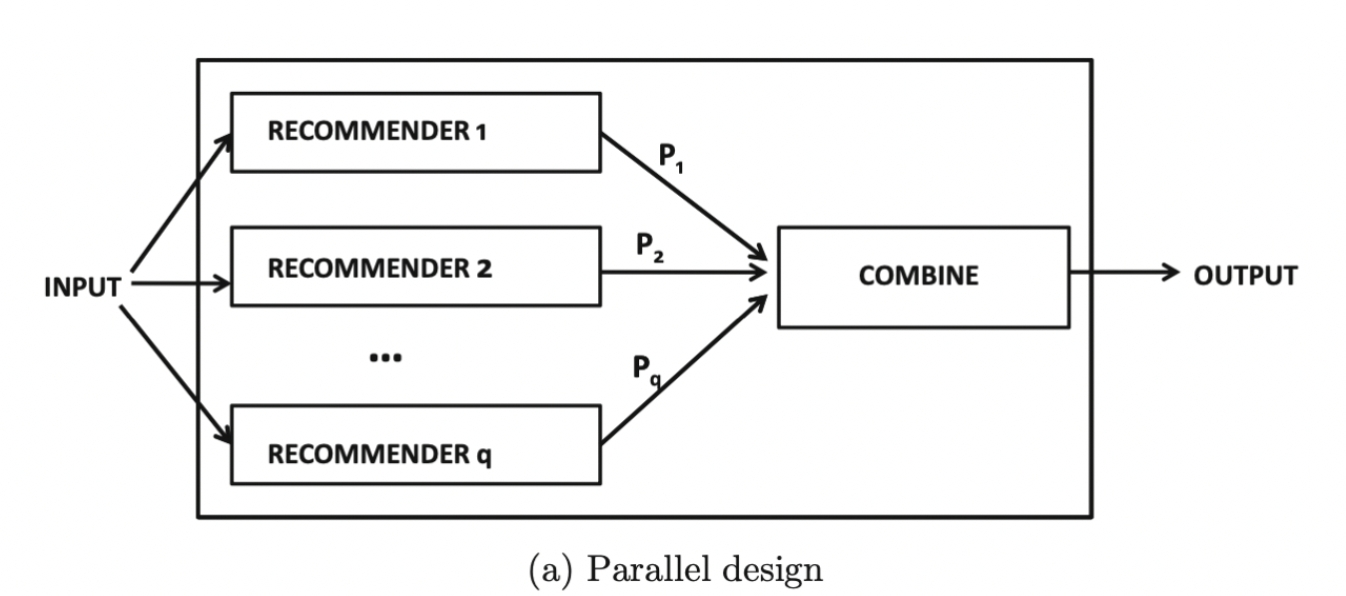
\includegraphics[scale = 0.5]{padesign}
% \caption{Parallel design of Hybrid Recommendation System}
% \centering
% \end{figure}
% \begin{figure}[ht]
% \centering
% 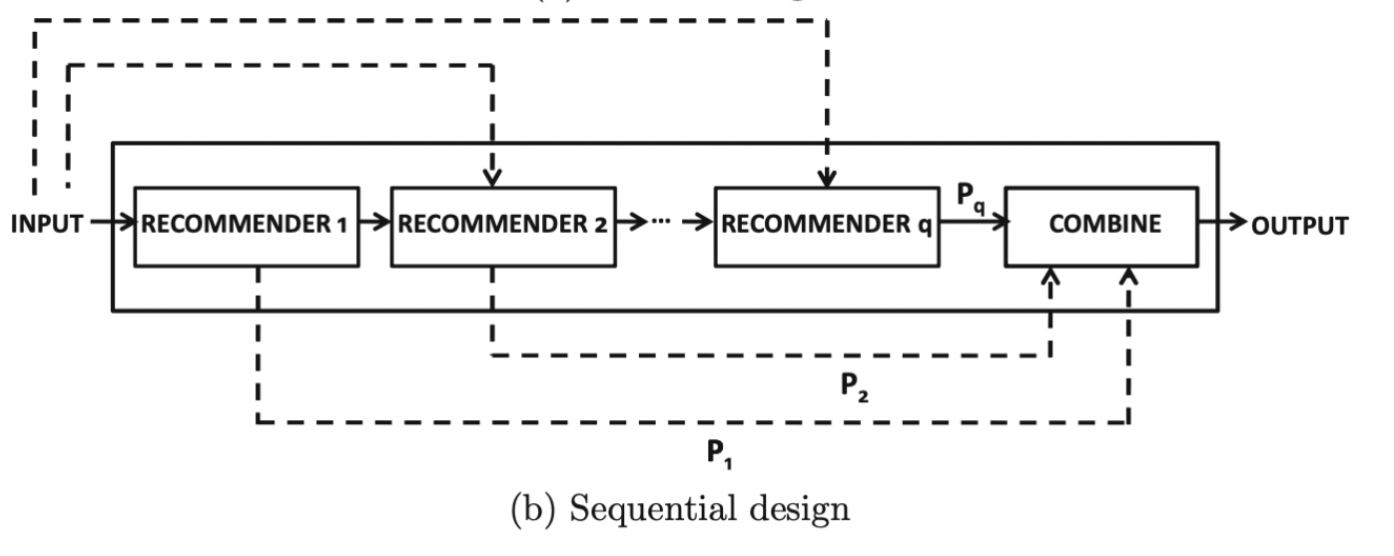
\includegraphics[scale = 0.5]{sedesign}
% \caption{Sequential design of Hybrid Recommendation System}
% \centering
% \end{figure}
\textbf{Advantages}
\\Hybrid systems combine different models to combat the disadvantages of one model with another. This overall reduces the weaknesses of using individual models and aids in generating more robust recommendations. This yields more robust and personalised recommendations for users.
\\\textbf{Disadvantages}
\\These types of models generally have high computational complexity and require a large database of ratings and other attributes to keep up to date. 
Without up to date metrics (user engagement, ratings, etc.) it makes it difficult to retrain and provide new recommendations with updated items and ratings from various users.

\section{Evaluation}
Identifying what defines a good recommendation is a problem in its self that many companies struggle with. This definition of “good” recommendations help evaluate the performance of the recommender you built. 
The quality of a recommendation can be assess through various tactics which measure coverage and accuracy. 
Accuracy is the fraction of correct recommendations out of total possible recommendations while coverage measures the fraction of objects in the search space the system is able to provide recommendations for. 
The method of evaluation of a recommendation is solely dependent on the dataset and approach used to generate the recommendation. 
Recommender systems share several conceptual similarities with the classification and regression modelling problem. 
In an ideal situation, we would want to see how real users react to recommendations and track metrics around the user to improve your recommendation, however, this is quite difficult to accomplish. 
Common statistical accuracy measures to evaluate accuracy of a recommender are RMSD, MAE, and k fold cross validation.

\subsection{K Fold Cross Validation}
This is one of the non-exhaustive validation methods, which means it does not compute all ways of splitting the original sample.
\begin{itemize}
\item Imagine you’ve built a model which will predict how well a user will rate an item based on a set of features. K fold cross validation can be used to infer the results of the model through accuracy metrics
\item Same idea as a train test split, except we create K many randomly assigned training and test sets
\item Each individual training set / fold is used to train on the recommendation system independently and then measure the accuracy of the resulting systems against the test set
\item We take the average of accuracy score to see how well the recommendation system is learning
\item This method is beneficial to prevent your model from overfitting, however it is a computationally extensive process
\end{itemize}

\subsection{Mean Absolute Error (MAE)}
Mean absolute error represents the average absolute value of each error in rating prediction
\begin{equation*}
\text{MAE} = \frac{\sum^{i=n}_{i=1}|y_{i} - x_{i}|}{n}
\end{equation*}
$y_{i}  = $ prediction
\\$x_{i}  = $ True Value
\\$n$ = total number of data points
\\Lower the MAE score the better.

\subsection{Root Mean Square Deviation(RMSD)}
\begin{equation*}
\text{RMSD} = \sqrt{\frac{\sum^{i=N}_{i=1}(y_{i} - x_{i})^{2}}{N}}
\end{equation*}

\begin{itemize}
\item A similar metric to MAE but has a stronger penalty for when the prediction is very far from the true value and weaker penalty for when the prediction is closer to the true value
\item Taking the squares off the difference of true and predicted values instead of the sum of the absolute values. This ensures that the resulting value is always positive and is larger when the difference is high and smaller when the difference is low.
\item The lower the RMSD score the better
\end{itemize}


\section{Implementation}
\subsection{System Design}
We finally decided to design our recommendation system using a hybrid system shown in \autoref{hybridd}. The system consists four sub-systems in parallel with each other, 
with one of the sub-systems is built with content-based and model-based filtering connected in series.
\begin{figure}[ht]
    \centering
    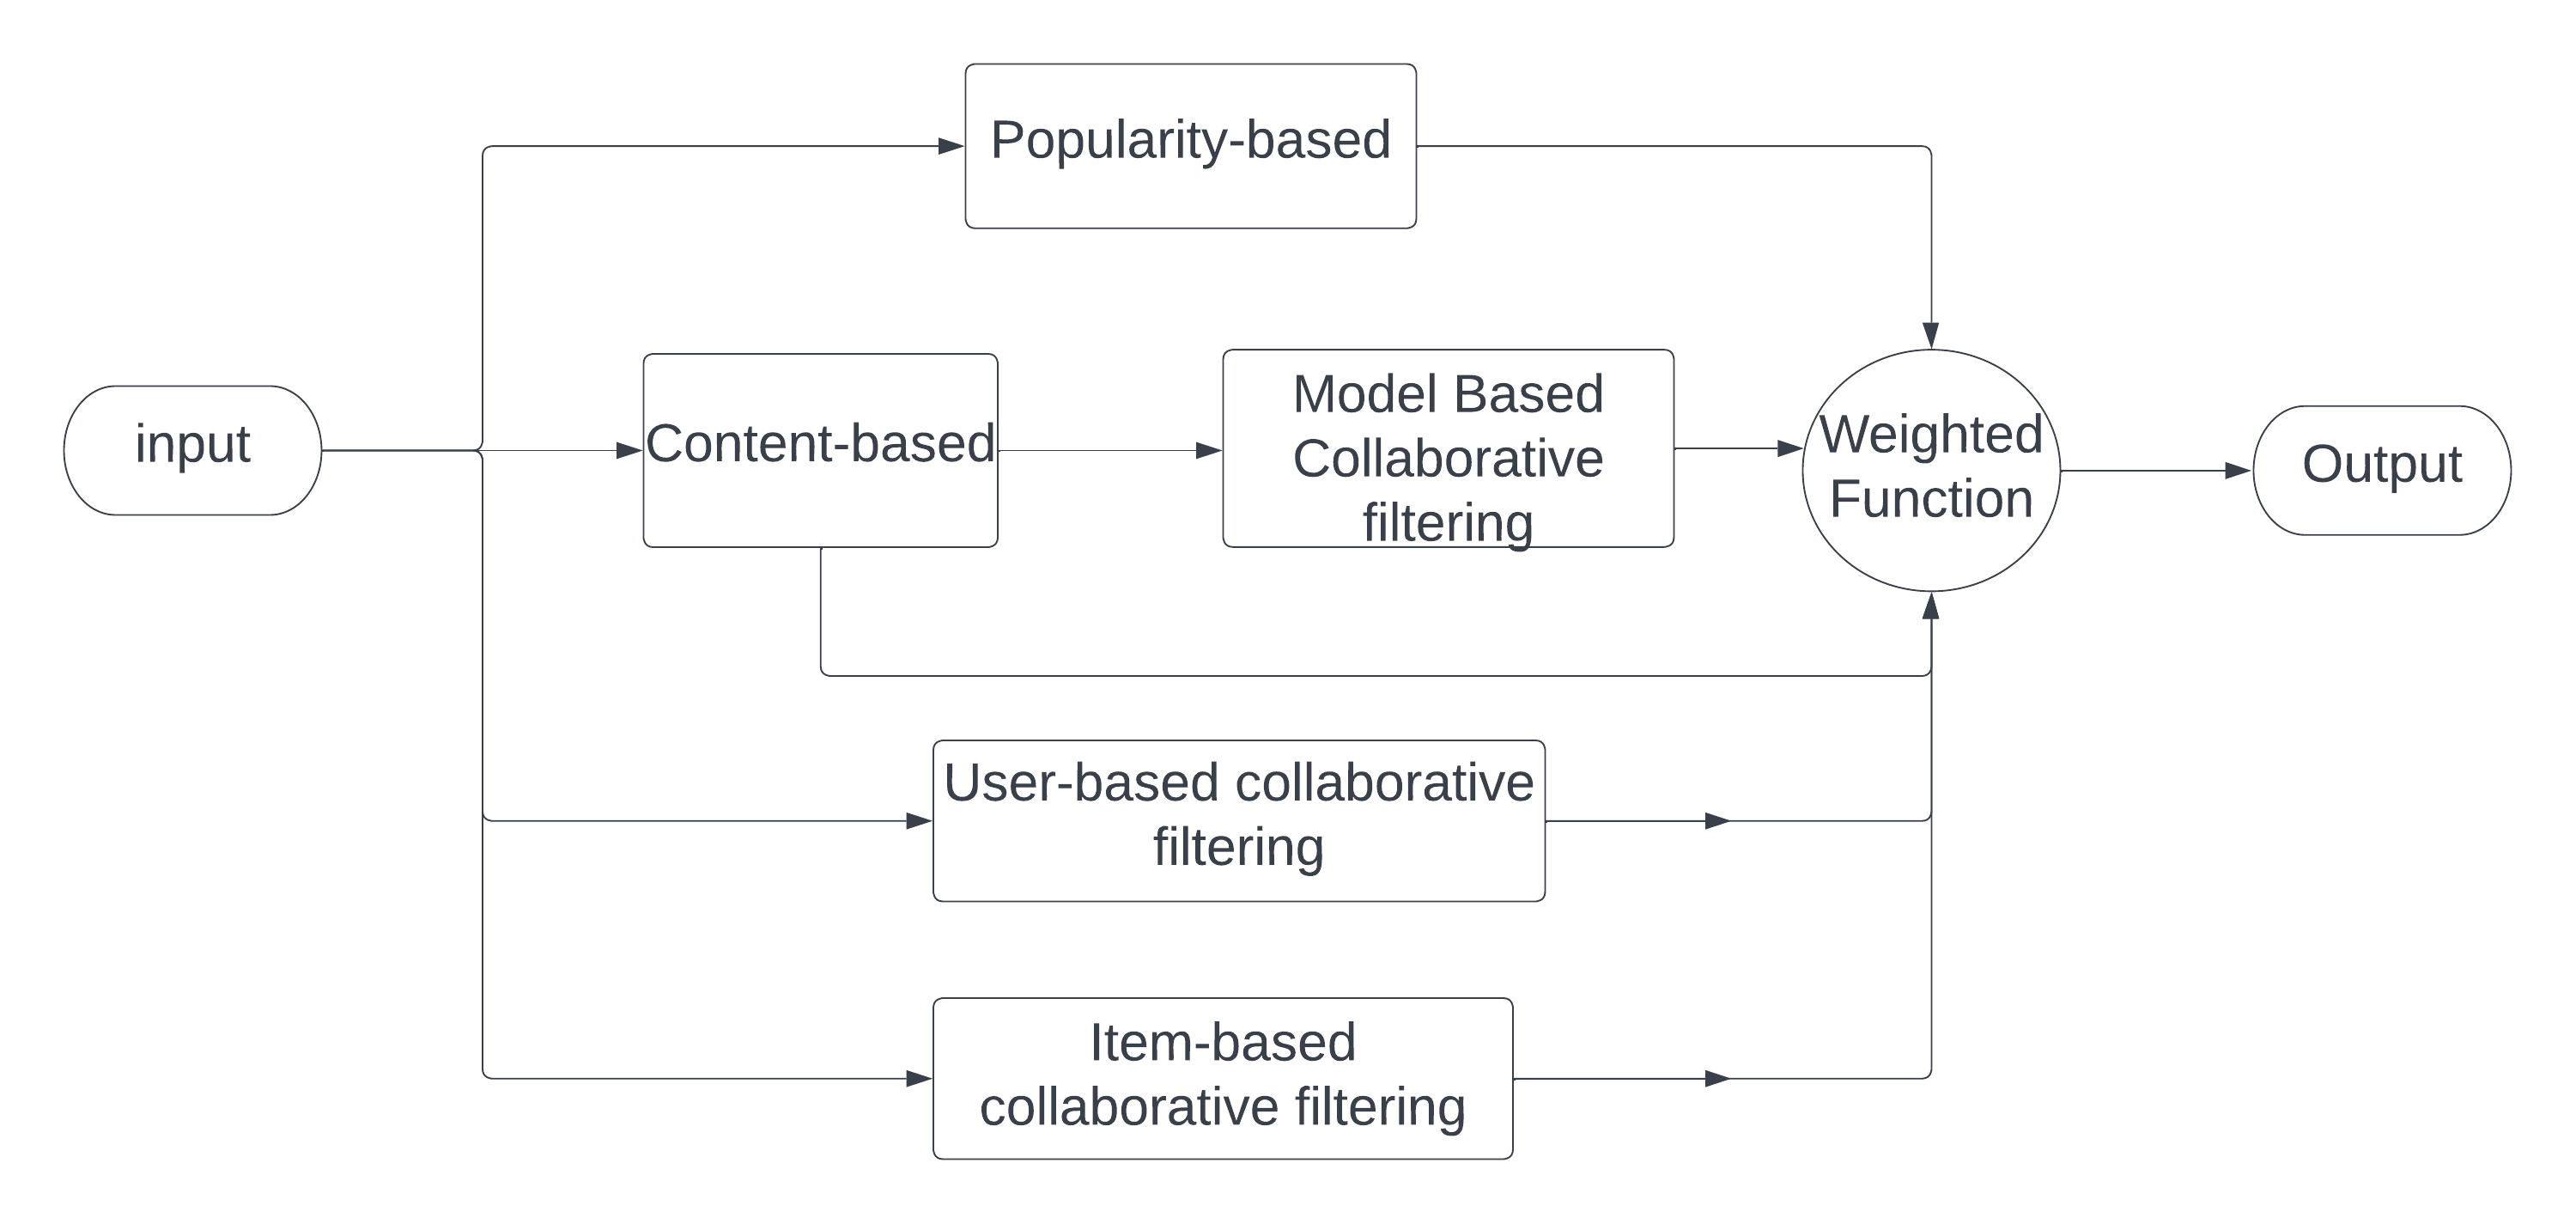
\includegraphics[scale = 0.15]{hybridd.png}
    \caption{Hybrid recommendation system design}
    \label{hybridd}
    \end{figure}
\\Firstly, the input which is information gathered from our users, will be passed through the popularity based system to get the ratings for their popularity.
\\In addition, the input will be feed into content-based system to have ratings based on the similarity between users' perference and posts' features. 
The reason why we also pass the output after the content-based system through a model-based collaborative filtering is to solve the limitations in last step, 
which are that users parameters vector can not be updated and users will not be recommended the type of posts if they have not interact with it before.
\\Furthermore, the input will pass through the user-based and item-based collaborative filtering system in parallel with other systems, 
to have the ratings of posts based on the analysis of group behaviors.
\\Finally after we have ratings after each system, we pass all the results into a weighting function, where we give weights to each sub-system output, and then apply a linear combination.
The weights coefficients are calculated based on the performance and reliability of the sub-systems.

\subsection{Top-k Recommendation}
\label{Top-k Recommendation}
In reality, we only care about the top-rated posts for our users. 
\\top-k explained here




